\documentclass[tikz, border=1mm]{standalone}
\newcommand{\FontPath}{../../../../../../../assets/fonts/} 
\usepackage{fontspec}
\usepackage{unicode-math}

% Thiết lập phông chữ
\setmainfont{STIX Two Text}
\setsansfont{STIX Two Text}
\setmonofont{STIX Two Text}
\setmathfont{STIX Two Math}


\usepackage{xcolor}
\definecolor{quartoText}{RGB}{33, 37, 41} % Màu văn bản chính từ theme default của quarto
    
\usepackage{tikz}
\usetikzlibrary{arrows, positioning, calc}

% Đảm bảo mọi nội dung trong tikzpicture đều dùng màu văn bản chính
\AtBeginEnvironment{tikzpicture}{\color{quartoText}}
\usepackage{pgfplots}
\pgfplotsset{compat=1.18}
\begin{document}
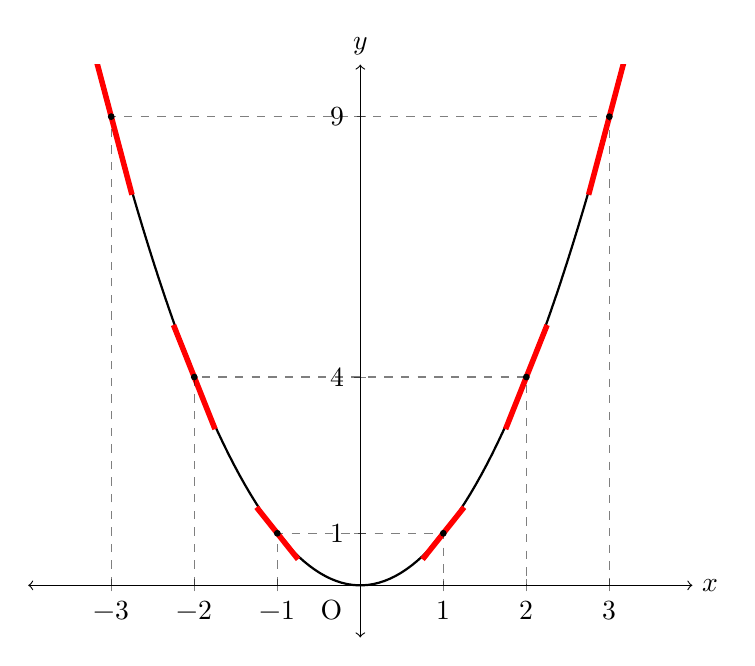
\begin{tikzpicture}
\begin{axis}[
    axis lines=middle,
    axis line style={<->},
    xlabel={$x$},
    ylabel={$y$},
    xlabel style={at={(axis cs:4,0)},anchor=west},
    ylabel style={at={(axis cs:0,10)},anchor=south},
    xmin=-4, xmax=4,
    ymin=-1, ymax=10,
    xtick={-3,-2,-1,0,1,2,3},
    ytick={0,1,4,9},
    % axis equal image,
    scale only axis,
    % width=10cm,
    % height=8cm,
]

\addplot[domain=-3.2:3.2, samples=100, thick] {x^2};
\node at (axis cs:-.1,-.1) [anchor=north east] {O};
\foreach \x in {-3,-2,-1,1,2,3} {
    \addplot[only marks, mark=*, mark size=1pt] coordinates {(\x,{(\x)^2})};
}

% Vẽ tiếp tuyến
\addplot[red, line width=2pt, domain=-1.25:-.75] {-2*x - 1};
\addplot[red, line width=2pt, domain=-2.25:-1.75] {-4*x - 4};
\addplot[red, line width=2pt, domain=-3.25:-2.75] {-6*x - 9};

\addplot[red, line width=2pt, domain=.75:1.25] {2*x - 1};
\addplot[red, line width=2pt, domain=1.75:2.25] {4*x - 4};
\addplot[red, line width=2pt, domain=2.75:3.25] {6*x - 9};


\draw [dashed, opacity=.5] (-1,0) -- (-1,1) -- (1,1) -- (1,0);
\draw [dashed, opacity=.5] (-2,0) -- (-2,4) -- (2,4) -- (2,0);
\draw [dashed, opacity=.5] (-3,0) -- (-3,9) -- (3,9) -- (3,0);


\end{axis}
\end{tikzpicture}
\end{document}
